
\documentclass[10pt,a4paper]{article}
\usepackage[utf8]{inputenc}
\usepackage[french]{babel}
\usepackage{listings}
\usepackage{graphicx}
\usepackage[left=2cm,right=2cm,top=2cm,bottom=2cm]{geometry}
\usepackage{hyperref}
%opening
\title{Le Protocole MQTT}
\author{Nicolas Vadkerti}
\usepackage{listings} % Required for inserting code snippets
\usepackage[usenames,dvipsnames]{color} % Required for specifying custom colors and referring to colors by name

\definecolor{DarkGreen}{rgb}{0.0,0.4,0.0} % Comment color
\definecolor{highlight}{RGB}{255,251,204} % Code highlight color

\lstdefinestyle{Style1}{ % Define a style for your code snippet, multiple definitions can be made if, for example, you wish to insert multiple code snippets using different programming languages into one document
language=Perl, % Detects keywords, comments, strings, functions, etc for the language specified
backgroundcolor=\color{highlight}, % Set the background color for the snippet - useful for highlighting
basicstyle=\footnotesize\ttfamily, % The default font size and style of the code
breakatwhitespace=false, % If true, only allows line breaks at white space
breaklines=true, % Automatic line breaking (prevents code from protruding outside the box)
captionpos=b, % Sets the caption position: b for bottom; t for top
commentstyle=\usefont{T1}{pcr}{m}{sl}\color{DarkGreen}, % Style of comments within the code - dark green courier font
deletekeywords={}, % If you want to delete any keywords from the current language separate them by commas
%escapeinside={\%}, % This allows you to escape to LaTeX using the character in the bracket
firstnumber=1, % Line numbers begin at line 1
frame=single, % Frame around the code box, value can be: none, leftline, topline, bottomline, lines, single, shadowbox
frameround=tttt, % Rounds the corners of the frame for the top left, top right, bottom left and bottom right positions
keywordstyle=\color{Blue}\bf, % Functions are bold and blue
morekeywords={}, % Add any functions no included by default here separated by commas
numbers=left, % Location of line numbers, can take the values of: none, left, right
numbersep=10pt, % Distance of line numbers from the code box
numberstyle=\tiny\color{Gray}, % Style used for line numbers
rulecolor=\color{black}, % Frame border color
showstringspaces=false, % Don't put marks in string spaces
showtabs=false, % Display tabs in the code as lines
stepnumber=5, % The step distance between line numbers, i.e. how often will lines be numbered
stringstyle=\color{Purple}, % Strings are purple
tabsize=2
}

\newcommand{\insertcode}[2]{\begin{itemize}\item[]\lstinputlisting[caption=#2,label=#1,style=Style1]{#1}\end{itemize}} 


% \insertcode{"Scripts/example.pl"}{Nena would be proud.} 

\begin{document}

\maketitle


\url{https://github.com/SlaynPool/CR_MQTT/}


\section{Le but de la seance}
Comme vu dans le compte rendu de la premier journée:
\url{https://github.com/SlaynPool/CR_MQTT/blob/master/CR_DAY_ONE/MQTT.pdf}
nous savons comment fonctionne le Protocole MQTT. Le but aujourd'hui est donc de mettre en place une infrastructure complete utilisant ce protocole.\\
Ainsi, nous allons déployer un broker MQTT, une base de donnée adapté aux besoins de l'IOT et un moyen de visualiser les données de la Base de donnée.
\section{Le broker MQTT}
Pour cette partie, nous allons utiliser Mosquito \url{https://mosquitto.org/}\\
Je n'ai pas configurer de mots de passe pour l'accés à notre broker ce qui fais que je n'ai pas eu a configurer le broker.
A noter,  tous les machines que nous allons utiliser dans ce CR seront des Debian 10.
\insertcode{commande/installBroker.txt}{Installation du broker}
On verifie que le broker fonctionne bien :

 \insertcode{commande/testbroker.txt}{Test du broker}
 
 
 \section{La base de donnée}
 
 Cette partie sera donc consacrée à comment nous allons récupérer les infos envoyer sur notre broker et comment nous allons les stocker. Il est sans doute bon de rappeller que le broker MQTT n'a pas pour rôle de stocker les données mais seulement de s'assurer de les livrers aux subscribers du topic. \\
 En pratique, si nous voulons stocker les données émis par nos capteurs, il faut que nous ayons un ``script/programme/plugin'' qui soit capable de se subcribe à tous les topics qui nous interesse, et faire les bonnes requetes SQL sur la bonne Base de Donnés pour les stocker 
 \subsection{Choix et déploiment de la base de Donnée}
 Nous voulons faire de l'IOT, on peut facilement supposer que nous allons potentiellement émettre beaucoup de petites données qui auront de la cohérence en fonction du temps. Un produit repondant à ce besoin éxiste et s'appelle InfluxDB. 
\begin{lstlisting}
InfluxDB is an open-source time series database (TSDB) developed by InfluxData.
It is written in Go and optimized for fast, high-availability storage and retrieval of
time series data in fields such as operations monitoring, application metrics, Internet
of Things sensor data, and real-time analytics. 

                            source: Wikipedia 
\end{lstlisting}
\subsubsection{Déploiment de InfluxDB}
Pour cela, j'ai suivi la documentation disponible sur le site de InfluxDB
\insertcode{commande/installinflux.txt}{Installation de InfluxDB}
De plus, pour pouvoir interagir avec notre base :
\insertcode{commande/installclient.txt}{Installation du client}
note: J'ai supprimer la VM entre la realisation des manipulations en cours et la redaction du compte rendu, j'ai donc recommemencé les manipulations sur une autre machines d'où l'incohérence des promptes
On verifie que l'on peut bien accéder à notre base :
\insertcode{commande/influx.txt}{accées à la base}

\section{Télégraf}
Nous allons maintenant nous intérésser à un outils très pratiques qui est Télégraf. En effet, il sert à lier notre base de données InfluxDB à differentes téchnologie, et dans notre cas present, un broker MQTT, aux travers de ``plugins'' dont une bonne partie est près installé . Son rôle va donc de se subcribe aux topics de notre broker, et de stocker les données dans la base. 
\subsection{Déploiment de Télégraf}
source: \url{https://portal.influxdata.com/downloads/}
\insertcode{commande/telegraf.txt}{Déploiment de télégraf}
Et pour ce qui est de la configuration : La commande diff n'est pas de moi mais trouvé sur internet. 
\insertcode{commande/telegrafconf.txt}{Configuration de télégraf}
J'ai donc configuré télégraf pour qu'il se subscribe à differents topics MQTT, et lui est préciser quelle type de valeurs il devait attendre.
Si on regarde dans notre base de donnés, il doit y avoir les données que nous donnons au broker, ici un Raspberry connécter à un accelerometre qui envoie les valeurs de celui-ci:
\insertcode{commande/pow.txt}{Preuve que Télégraf fonctionne}


\section{Visualiser les données}
Nous sommes capables d'éméttre nos données, nous somme capable de les stocker, il nous reste donc plus qu'a les visualiser via une interface Web par exemple. Une solution très efficase et bien documenté est Grapfana. Grapfana est capable de se connécter à une base Influxdb et de générer des graphiques à partir de celui-ci.
\subsection{Déploiment de grafana}
source: \url{https://grafana.com/docs/grafana/latest/installation/debian/}
\insertcode{commande/grafanainstall.txt}{installation de grafana}
On peut donc verifier que grafana fonctionne bien:
  \begin{figure}[h!]
\centering
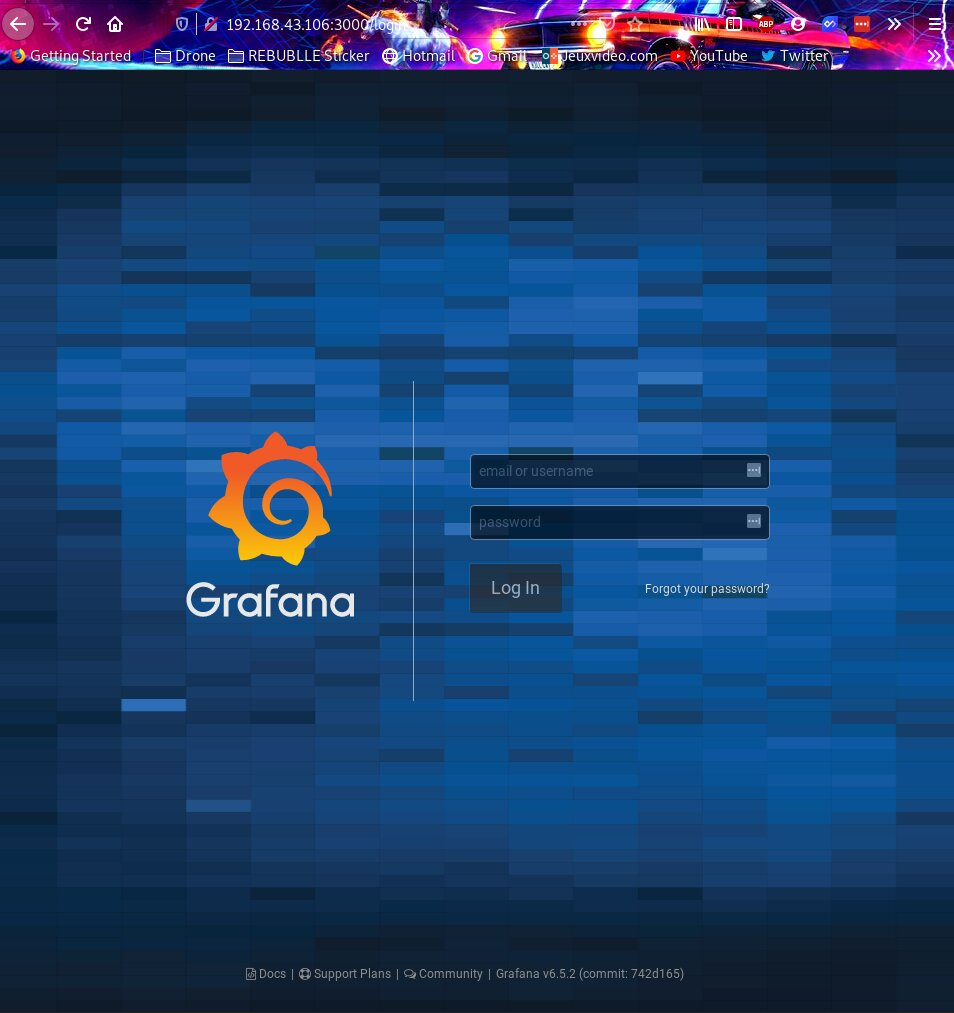
\includegraphics[scale=0.30]{screen/1.jpg}
\caption{Interface}
\label{fig:net }
\end{figure}
\\On peut donc ce connecter avec les mots de passes par default: `` admin'' ``admin`` et configurer les data sources comme ceci dans notre cas:
  \begin{figure}[h!]
\centering
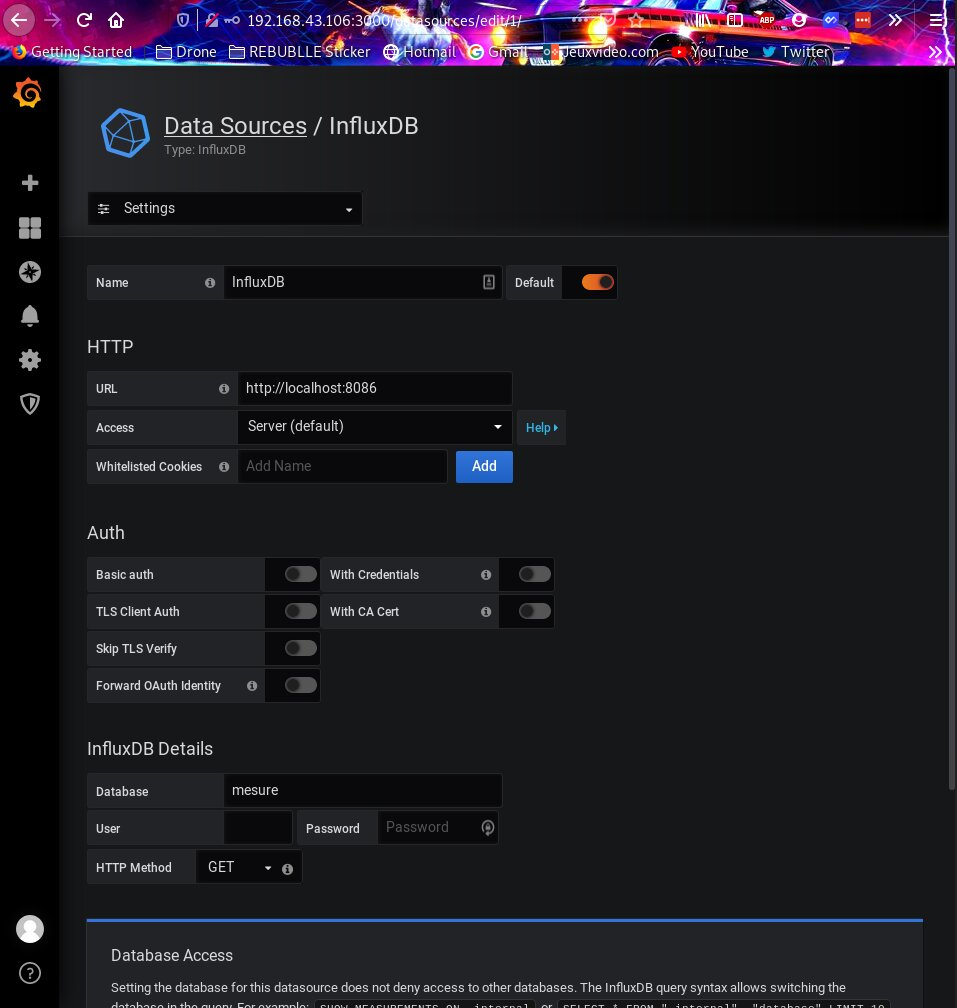
\includegraphics[scale=0.50]{screen/2.jpg}
\caption{Network Schema}
\label{fig:net }
\end{figure}
\\On sauvegrade celle-ci. Quand nous sauvegardons, il grafana essaye desuite de ce connecter à la base de donné donc nous savons directement si elle est correctement configuré ou non. \newpage 

Des lors, nous pouvons configurer nos nouveaux dashboards comme ci dessous:
  \begin{figure}[h!]
\centering
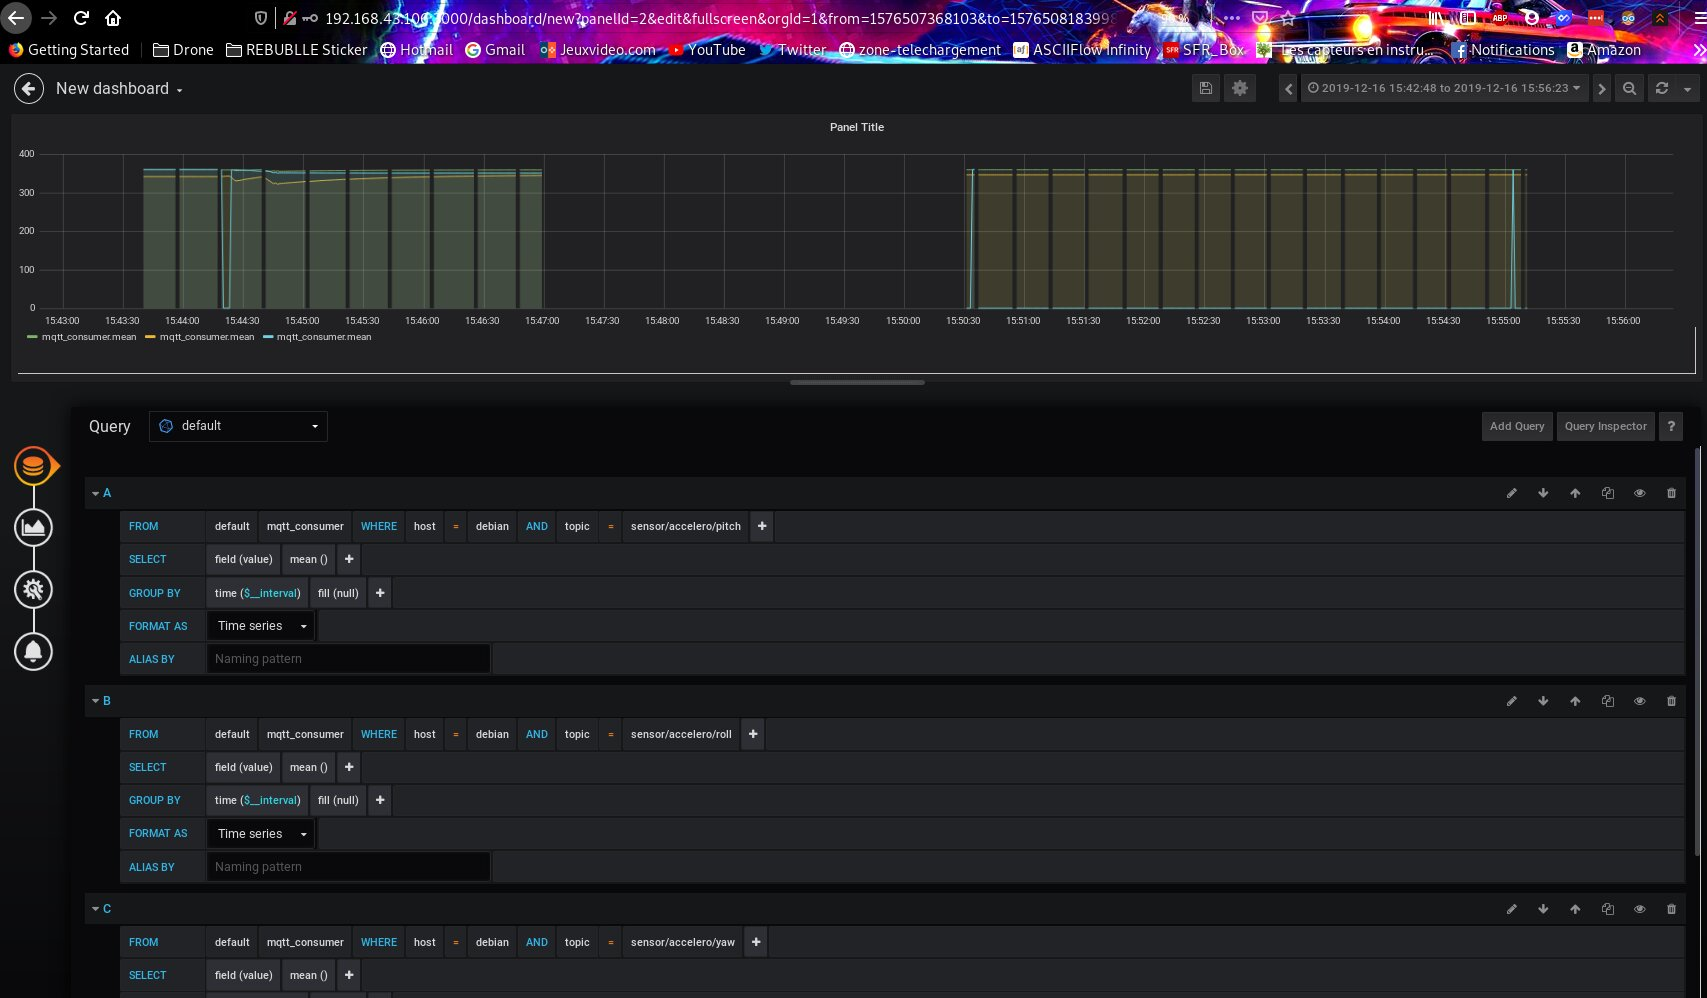
\includegraphics[scale=0.50]{screen/3.jpg}
\caption{Network Schema}
\label{fig:net }
\end{figure}
\\ Il suffit de lui donner les bonnes requetes (ce qui via l'interface est très intuitif par ailleur) et il génére le grafique qui va bien. 



\end{document}

